\section{Correspondence Analysis for Approximating Political Ideology\label{sec:appendix-ca}}
After identifying our set of 882 politically discriminating and identifying 7,7 random accounts that followed this set of accounts, we performed the following for CA. 

\begin{enumerate}
\item{\textbf{Identify the Ideological Subspace:}} Using 6,107 accounts that followed 10 or more of our 882 discriminating political users, we derive an initial CA model and obtain a discriminating latent space on which to plot user political ideology. 

\item{\textbf{Expand the number of discriminating political ideological accounts:}} Utilizing our initial CA model we determine the set of Twitter accounts not included within our initial target accounts that were most often followed by the most conservative and liberal accounts (within the top 20\% on either side of the political spectrum) in the first stage of our analysis. As in Barbera et~al.~\cite{barbera2015tweeting}, we compute the popularity among users of a given ideological orientation such that $pop_{jc} = n_{jc} -  n_{jl}$  for conservatives, where $n_{jc}$ is the number of conservative users included in the first stage
that follow account j, and $n_{jl}$ is the equivalent measure for liberals. We further filter these accounts to ensure that at least 3r different users follow these additional discriminating accounts. After determining these users, we add the resulting 788 accounts as additional "following" accounts to our original $n \times m$ matrix. These additional accounts include those of Barack Obama (@BarackObama), MSNBC (@MSNBC), Florida governor Ron Desantis (@GovRonDeSantis), and the House GOP (@HouseGOP).

\item{\textbf{Expanding the number of follower accounts:}} For the rest of our users, we project them into the discriminating latent space utilizing our CA model. This allows us to utilize the information from our original discriminating political accounts as well as from the additional discriminating political accounts from the second stage. We further can estimate the political ideology of any account that follows at least one of 1607 highly politically discriminating accounts. After projecting all of our users we standardize the estimates into z-scores  (\textit{i.e.,} a value of 0 represents the average partisanship and a value of 1 represents one standard deviation above the mean, 2, two standard deviations above the mean, \textit{etc...}). Altogether we project an additional 49,308 users. 

%Using the \texttt{tweepy} API, we then identify which,

\end{enumerate}

\section{Unsupervised Contrastive Learning\label{sec:finetune}}
We utilize the SimCSE training objective to further refine our MPNet model and ensure that it is properly suited for our dataset. This is such that we embed each tweet $i$  $x_i = (tweet_i) \in D_{tweets}$ (where $tweet_i$ is the text) twice (with dropout both times) using MPNet by inputting $[CLS] text_i [SEP]$ and outputting out the contextual hidden vectors $\mathbf{h}_i$ and $\tilde{\mathbf{h}}_i$  for $text_i$ as its representations. Then, given a batch of contextual hidden vectors $\{\mathbf{h}_i\}_{i=0}^{N_b}$ and $\{\tilde{\mathbf{h}}_{j}\}_{j=0}^{N_b}$ (different dropout), where $N_b$ is the size of the batch, for each batch in our training dataset of 1 million tweets, we perform a contrastive learning step on that batch. This is such that for each batch $\mathcal{B}$, for an \textit{anchor} hidden embedding $\mathbf{h_i}$ within the batch, the set of hidden contextual vectors $\mathbf{h_i} \, \mathbf{\tilde{h_j}} \in \mathcal{B}$, 
 the hidden contextual vectors where $i = j$ are positive pairs. Other pairs where $i\neq j$ are considered negative pairs. Within each batch $\mathcal{B}$, the contrastive loss is computed across all positive pairs in the batch such that:
\[
    L_{contrastive} = -\frac{1}{N_b} \sum_{\mathbf{h}_i \in \mathcal{B}}\mathit {l}^c(\mathbf{h}_i )
\]
\[
\mathit{l}^c(\mathbf{h}_i) = {log}\frac{ \sum_{j\in\mathcal{B} } \mathbbm{1}_{[i = j]}\mathrm{exp}( \frac{\mathbf{h}_i^\top \tilde{\mathbf{h}_j}}{\tau||\mathbf{h}_i || ||\tilde{\mathbf{h}_j} || })}{\sum_{j\in\mathcal{B}} \, \mathrm{exp}( \frac{\mathbf{h}_i^\top \tilde{\mathbf{h}_j}}{\tau||\mathbf{h}_i || ||\tilde{\mathbf{h}_j} || })}
\]
where, as in prior work~\cite{liang2022jointcl}, we utilize a temperature $\tau=0.07$.


\section{Training our Open-Source Toxicity Classifier\label{sec:app-tox-classifier}}

\vspace{2pt}\noindent
\noindent
\textbf{Realistic Adversarial Perturbations of the Civil Comments Training Dataset.} To train our model, we rely on the Civil Comments training dataset which consists of 1,804,874~comments that were each individually graded by up to 10~human raters for their toxicity. Each comment, depending on the percentage of human raters that graded the comment as ``toxic'' (toxic having the definition provided in Section~\ref{sec:misinformation-defintion}), is assigned a score between 0 and 1. Our  training dataset is thus $D_{Civil} = \{x_i = (text_i,t_i)\}^N_{i=1}$, where $text_i$ a text, and $t_i$ is the toxicity of the text. While the Civil Comments training dataset is fairly large, we note that it is heavily skewed with 1,268,269 of the comments having a toxicity score of 0. To ensure that our training dataset has a wider set of examples of comments with above zero estimated toxicity, we augment the Civil Comments training dataset using realistic adversarial perturbations~\cite{le2022perturbations}. 


Utilizing the ANTHRO dataset provided by Le  {et~al.}~\cite{le2022perturbations}, for every comment with above zero toxicity within the Civil Comments dataset, we leverage the set of common human-written perturbations to augment our Civil Comments dataset. This ANTHRO dataset consists of common online perturbations of words (\textit{e.g.}, Republican $\rightarrow$ republiican, Reeepublican, Republicaan) extracted from online texts (\textit{e.g.}, Twitter). For each comment with a toxicity score greater than zero in the Civil Comments training set, we extract a set of random perturbations of each noun and adjective within the comment, perturbing the overall comment nine times with different combinations of the perturbed nouns and adjectives. This enables us to extend the set of non-zero comments to a total of 5,366,050~comments (6,634,319 in the full augmented dataset). We utilize this dataset when training our DeBERTa-based~\cite{he2022debertav3} model to determine the toxicity of tweets. We note that in addition to allowing our model to have more training instances of toxic texts, this approach further enables our model to have training instances of real ``in-the-wild'' perturbations and misspellings of words that are often found on social media (\textit{e.g.}, Twitter) and online.




\vspace{2pt}\noindent
\noindent
\textbf{DeBERTa-based Contrastive Embedding Layer.} Besides utilizing our augmented dataset of realistic adversarial perturbations, while training our model, we pre-train a contrastive layer to differentiate toxic and non-toxic texts. We later freeze this layer while training our full model to identify the toxicity of individual tweets.


To pre-train this layer for use in our model, we utilize contrastive learning to differentiate toxic and non-toxic texts. As in the original Civil Comments task, while training this layer we consider texts with labeled toxicity $t_i$ $>0.5$ score in the Civil Comments dataset as toxic and those with labeled toxicity $t_i$ $<0.5$ as nontoxic. We utilize this threshold for classifying a comment as toxic, given that this score (as described in the Civil Comments task) indicates that a majority of the Civil Comments annotators would have assigned a ``toxic'' attribute to this comment. For training, this is such that we embed each example $x_i = (text_i,t_i) \in D_{Civil_{aug}}$ (where $text_i$ is the text and $t_i$ is whether the text is toxic or not) using a contextual word model by inputting $[CLS] text_i [SEP]$ and outputting the hidden vector $\mathbf{h}_i$ of the [CLS] token for each $text_i$ as its representation. Then, given a set of hidden vectors $\{\mathbf{h}_i\}_{i=0}^{N_b}$, where $N_b$ is the size of the batch, we perform a contrastive learning step on that batch. This is such that for each Batch $\mathcal{B}$, for an \textit{anchor} hidden embedding $\mathbf{h_i}$ within the batch, the set of hidden vectors $\mathbf{h_i} \,, \mathbf{h_j} \in \mathcal{B}$ vectors where $i \neq j$, we consider them a positive pair if $t_i, t_j$ are equivalent. Other pairs where $t_i\neq t_j$ are considered negative pairs. Within each batch $\mathcal{B}$, the contrastive loss is computed across all positive pairs in the batch such that:

\[
    L_{toxic} = -\frac{1}{N_b} \sum_{\mathbf{h}_i \in \mathcal{B}}\mathit {l}^c(\mathbf{h}_i )
\]
\[
\mathit{l}^c(\mathbf{h}_i) = {log}\frac{ \sum_{j\in\mathcal{B}\setminus i } \mathbbm{1}_{[t_i = t_j]}\mathrm{exp}( \frac{\mathbf{h}_i^\top \mathbf{h}_j}{\tau||\mathbf{h}_i || ||\mathbf{h}_j || })}{\sum_{j\in\mathcal{B}\setminus i } \, \mathrm{exp}( \frac{\mathbf{h}_i^\top \mathbf{h}_j}{\tau||\mathbf{h}_i || ||\mathbf{h}_j || })}
\]
\begin{figure}
\begin{minipage}[l]{0.5\textwidth}
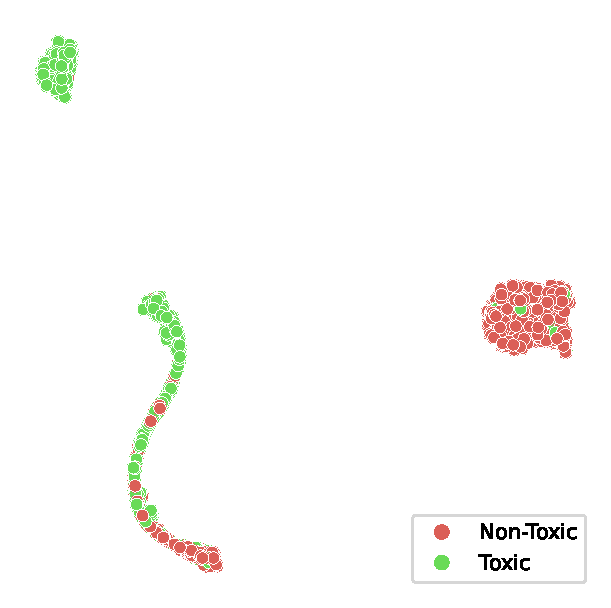
\includegraphics[width=1\columnwidth]{figures/toxicity_training_tsne.pdf} 
\end{minipage}
\begin{minipage}[l]{0.35\textwidth}
\caption{\textbf{t-SNE of Civil Comments Validation Dataset }-- As we train the DeBERTa-based contrastive embedding layer of our model on our augmented Civil Commonents training set, our model can differentiate non-toxic (\textit{i.e.,} toxicity $t_i < 0.5$) and (\textit{i.e.,} toxic $t_i > 0.5$) comments. However, comments that are of ambiguous toxicity are more difficult to differentiate.\label{figure:tsne} }
\end{minipage}

\end{figure}



\noindent
where, as in prior work~\cite{liang2022jointcl}, we utilize a temperature $\tau=0.07$. Throughout training, we use a batch size of 64 and a learning rate of $1\times 10^{-5}$, training for three epochs. After training this layer, we freeze it for use in the rest of our model. As seen in Figure~\ref{figure:tsne}, reducing the dimensionality of the outputted $h_{constrat}$ on the Civil Comments validation dataset using t-SNE~\cite{van2008visualizing}, our contrastive embeddings are largely though imperfectly, able to differentiate between non-toxic and toxic comments.

\vspace{2pt}\noindent
\noindent
\textbf{Full DeBERTa Toxicity Detection Model.} Taking our pretrained-DeBERTa contrastive embedding layer and our augmented dataset $D_{Civil_{aug}}$, we finally train our full DeBERTa toxicity detection model (Figure~\ref{fig:toxicity-twitter-model}. This model first computes the scaled dot product of a DeBERTa hidden representation of a text $h_{text}$ and the $h_{contrast}$ output of our DeBERTa contrastive embedding layer. The intuition behind this approach is to enable our model to determine the extent of the toxicity features present within the original text.  

\begin{align*}
r_{contrast} &= \sum_i a_ih_{text}^{(i)},\\
a_i &= \textrm{softmax} \left( \lambda h_{text}^{(i)} \cdot (W_{contrast} h_{contrast}) \right)
\end{align*}

\noindent
where and $\lambda = 1/\sqrt{E}$, $E=$ dimentionality of the the embeddings, and $W_{contrast}$ is a learned parameter matrix. Finally, once $r_{contrast}$ is calculated, we concatenate it using a residual connection with the original $h_{text}$. We then feed the resulting representation into a feed-forward network with ReLU activation for determining the toxicity of the text as seen in Figure~\ref{fig:toxicity-twitter-model}. We minimize mean squared error while training, utilizing the Civil Comments validation dataset to perform early stopping with a patience of 2. Throughout training, we use a batch size of 64 and a learning rate of $1\times 10^{-5}$. We completed all training on a Nvidia A6000 GPU\@. 

\begin{figure}
\begin{minipage}[l]{0.5\textwidth}
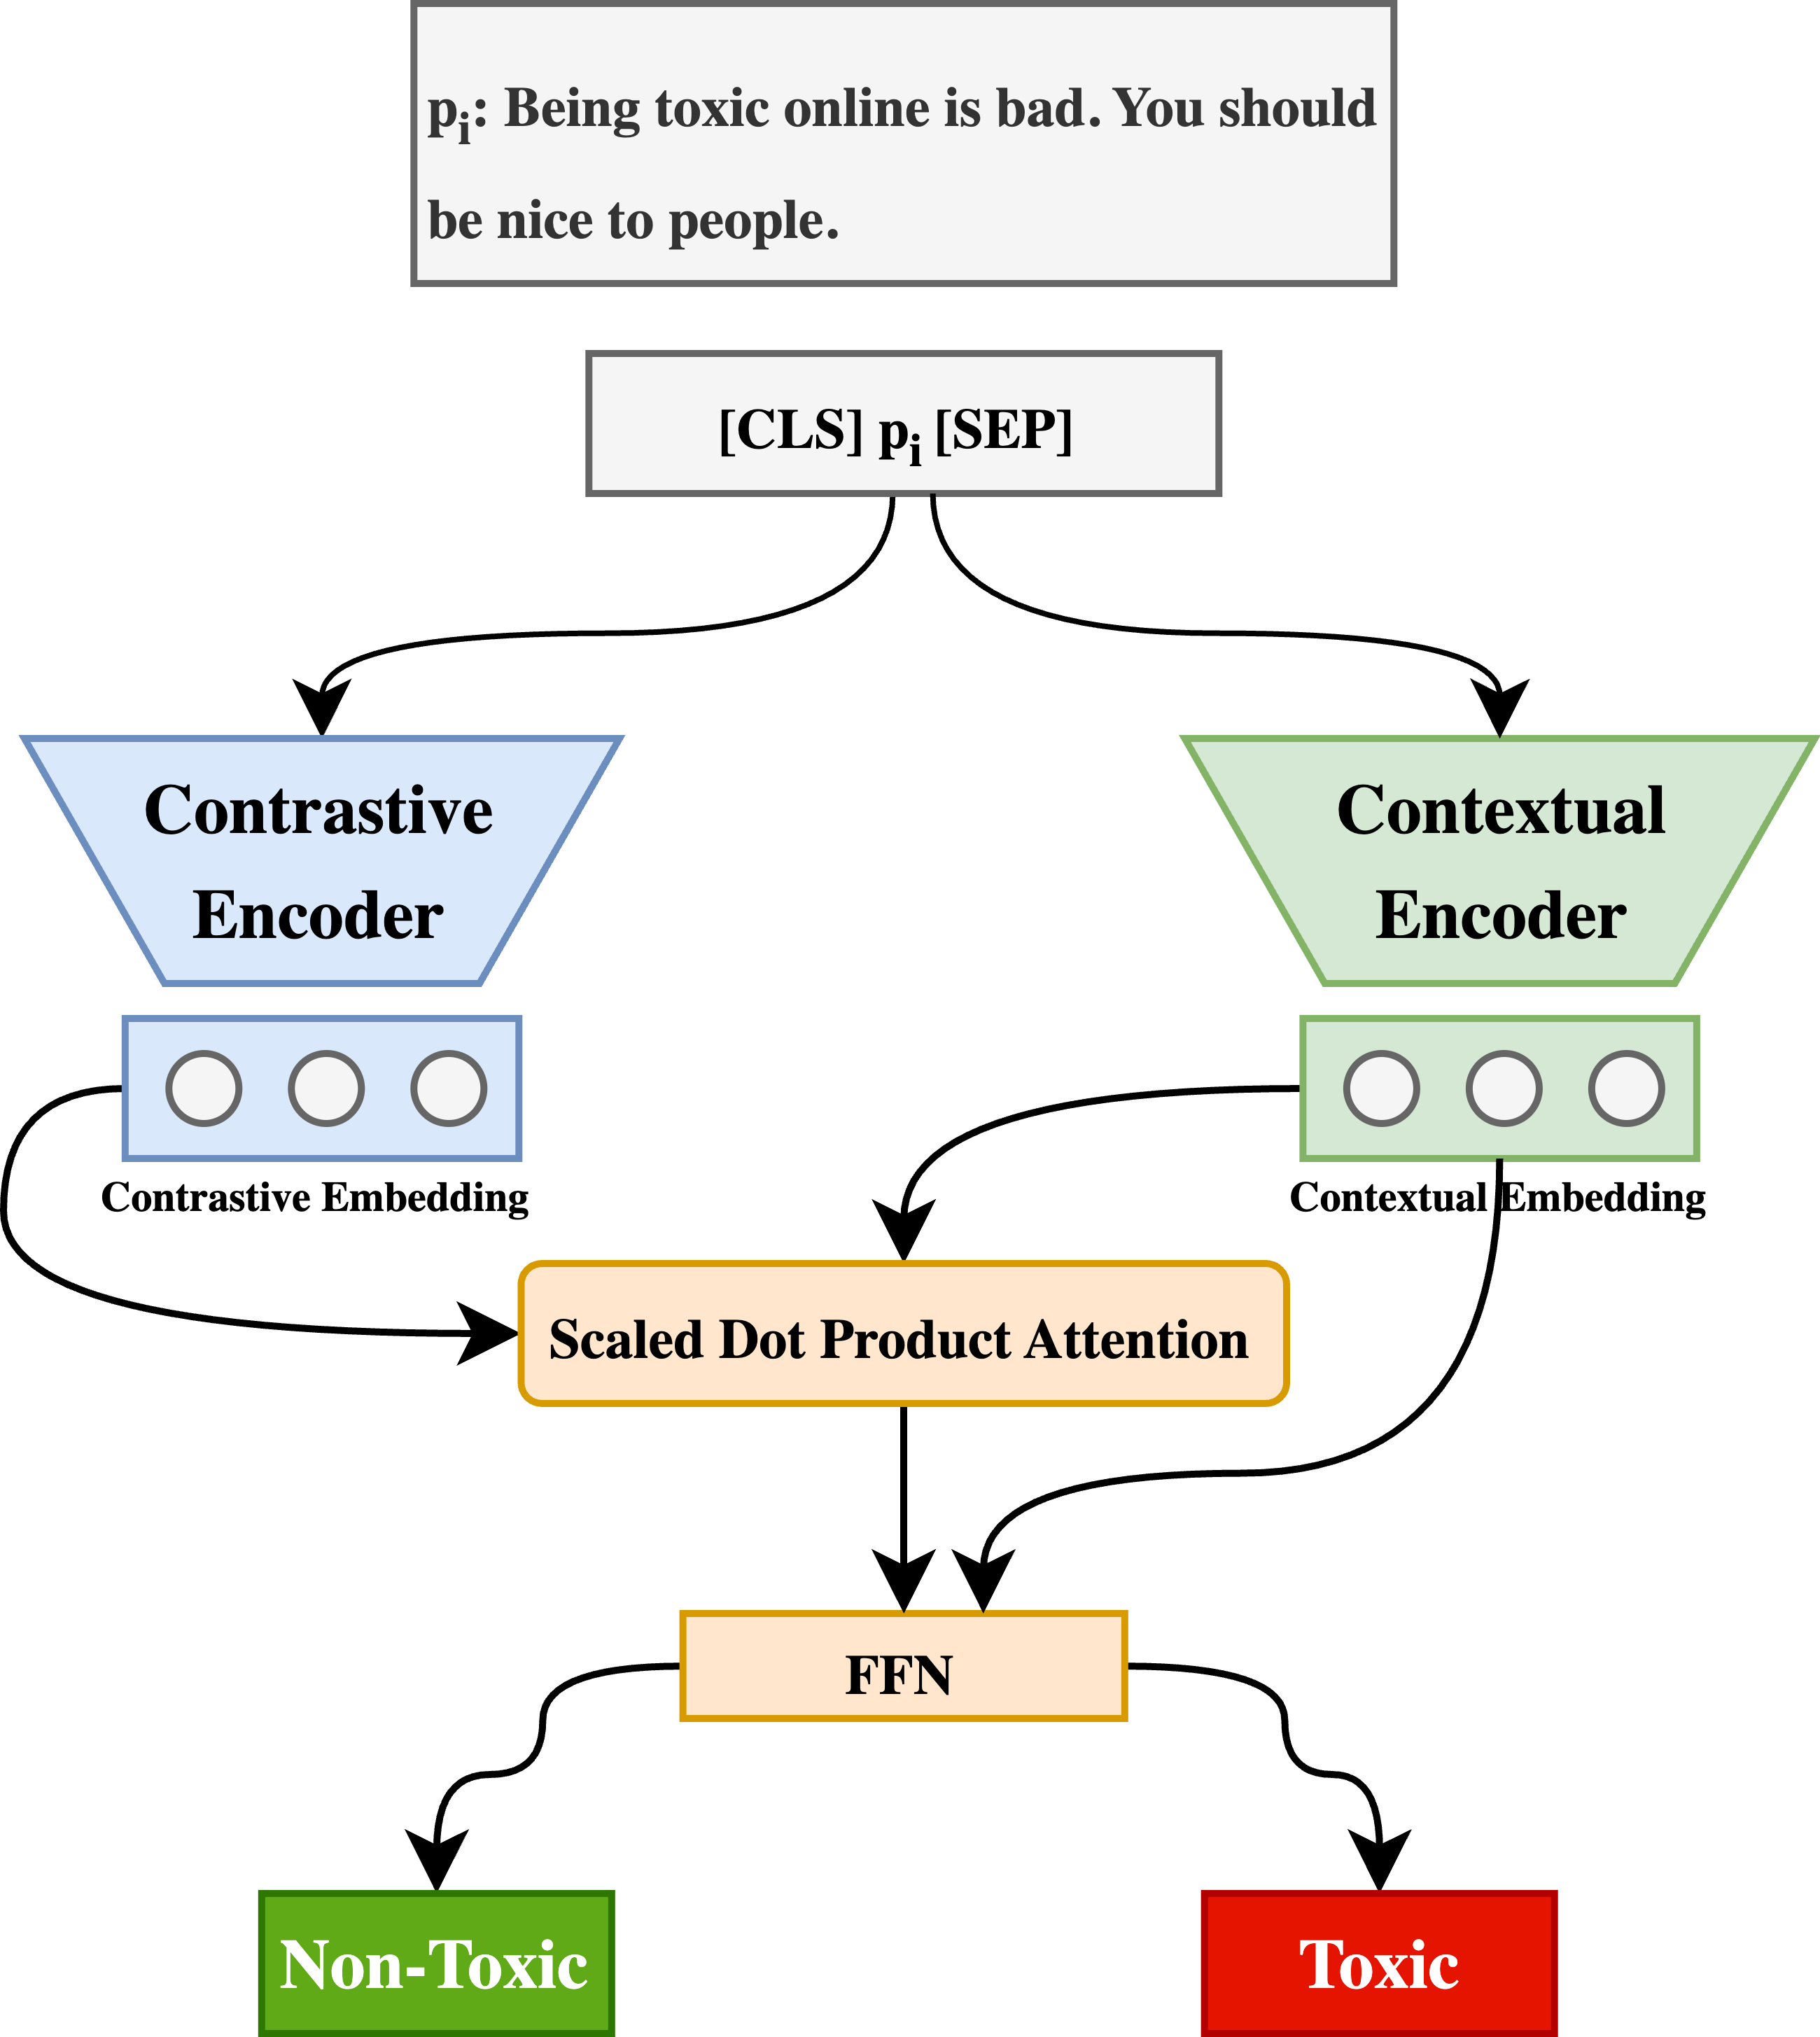
\includegraphics[width=1\columnwidth]{figures/toxicity_classification.drawio.png} 
\end{minipage}
\begin{minipage}[l]{0.35\textwidth}
\caption{{Model to determine the toxicity of individual tweets}--- We utilize contrastive learning, scaled-dot-product attention, and the DeBERTa model to train a model to predict the toxicity of tweets in our dataset. Our fully trained model achieves a 0.818 Pearson correlation with the toxicity scores in the Civil Comments test dataset. \label{fig:toxicity-twitter-model}}
\end{minipage}

\end{figure}


\section{Pointwise Mutual Information\label{sec:pmi} }

The pointwise mutual information PMI of a particular word $word_i$ in a cluster $C_j$ is calculated as:

\vspace{-10pt}
\begin{align*}
\scriptsize
PMI(word_i, C_j) = log_2\frac{P(word_i,C_j)}{P(word_i) P(c_i)}
\end{align*}
\vspace{-10pt}

\noindent where $P$ is the probability of occurrence and a scaling parameter $\alpha$ is added to the counts of each word. This scaling parameter $\alpha$ prevents single-count or one-off words in each cluster from having the highest PMI values. Given the scale of our dataset and the number of clusters within our dataset, we determine that a baseline count of 1 ($\alpha$ =1) for each word in the full dictionary in each cluster led to the best results~\cite{turney2001mining}. 


\section{DP-Means\label{sec:ap-dpmeans}}

DP-Means~\cite{kulis2011revisiting} is a non-parametric extension of the K-means algorithm that does not require the specification of the number of clusters \textit{a priori}. Within DP-Means, when a given datapoint is a chosen parameter $\lambda$ away from the closest cluster, a new cluster is formed. Dinari {et~al.}~\cite{dinari2022revisiting} parallelize this algorithm by \textit{delaying cluster creation} until the end of the assignment step. Namely, instead of creating a new cluster each time a new datapoint is discovered, the algorithm determines which datapoint is furthest from the current set of clusters and then creates a new cluster with that datapoint. By delaying cluster creation, the DP-means algorithm can be trivially parallelized. Furthermore, by delaying cluster creation, this version of DP-Means avoids over-clustering the data (\textit{i.e.,} only the most disparate data points create new clusters)~\cite{dinari2022revisiting}.

\clearpage
\newpage
\section{GAM Fit of of User-Level Features and Perspective Toxicity\label{sec:perspective-user-app}}
\begin{figure}[!h]
\begin{minipage}[l]{1.0\textwidth}
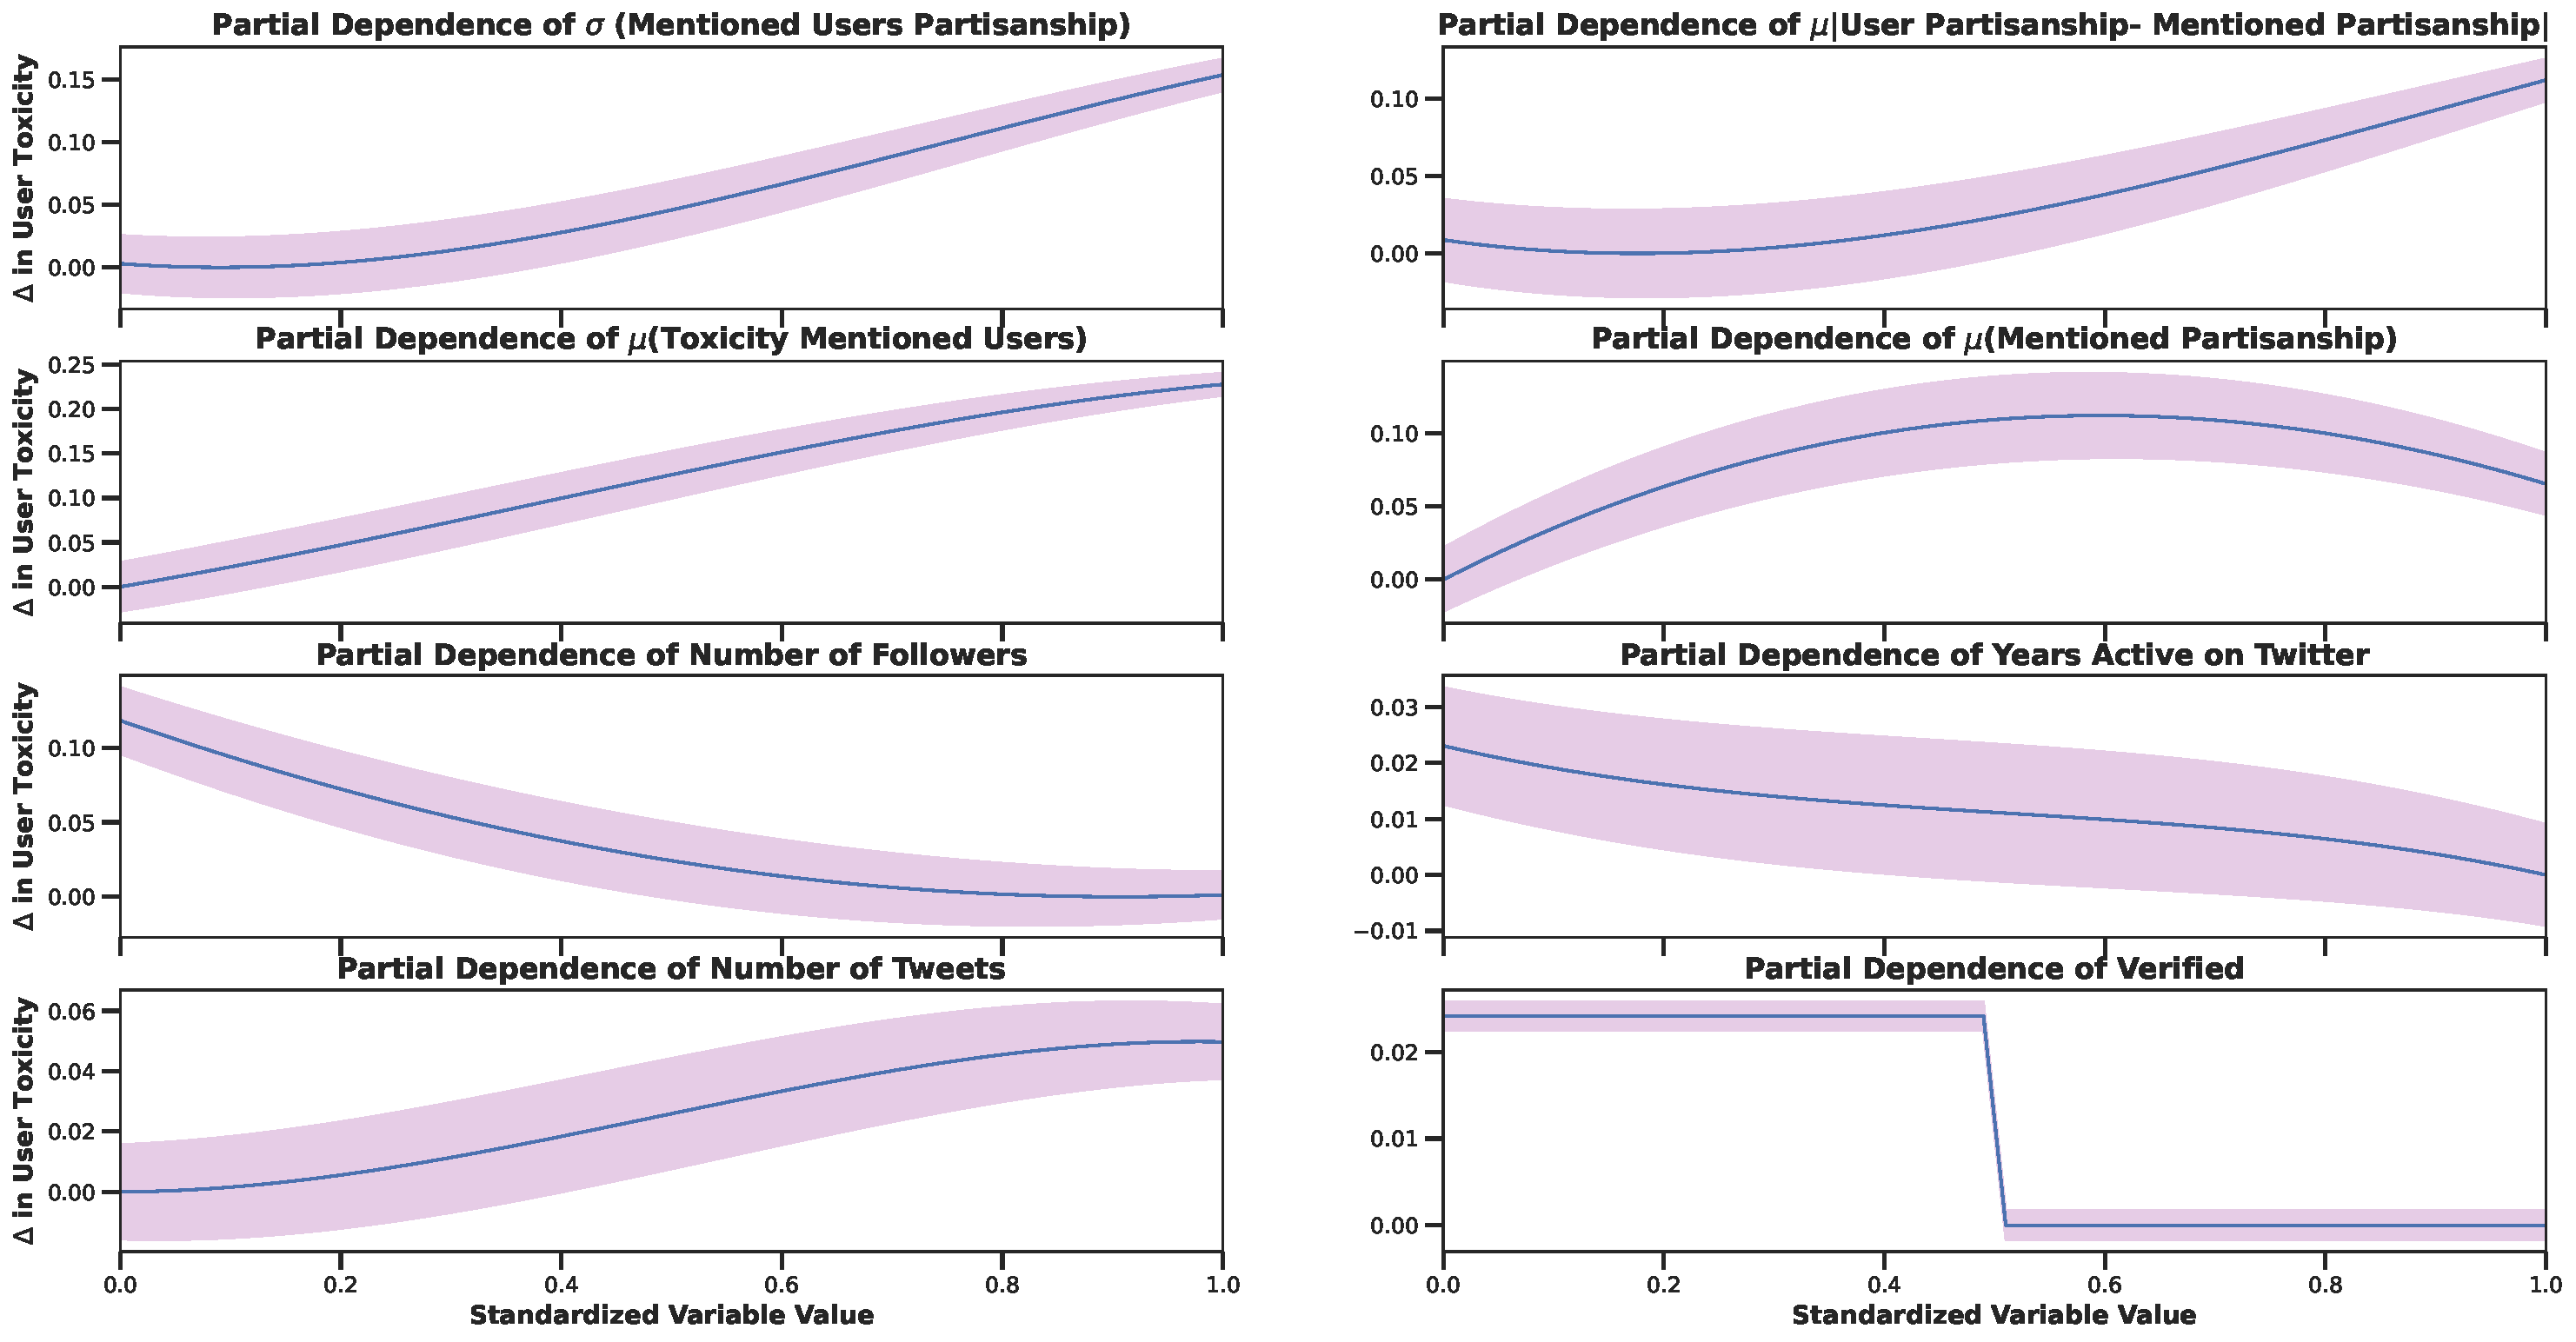
\includegraphics[width=1\columnwidth]{figures/partial_dependence_important_variables-perspective.pdf} 
\end{minipage}
\begin{minipage}[l]{1\textwidth}
\caption{Partial dependencies with 95\% Normal Confidence intervals between fitted standardized dependent variables and user Perspective API toxicity.}
\end{minipage}

\end{figure}

\begin{table}[!h]
    \small
    \centering
    \begin{tabularx}{0.9\columnwidth}{l|rrr}
    Train $R^2$ 0.266, Validation $R^2$:  0.270 \\
    \toprule
      Dependent Variable  & Pearson Corr. $\rho$ & Kendall's $\tau$ & Permut Import. \\    \midrule
  Verified Status & ---- &-0.233& 0.031  \\
  Years Active on Twitter & -0.220& -0.155 & 0.022 \\
  Log \# Followers & -0.229 &-0.137 & 0.231  \\
  Log \# Followed & -0.197 & -0.128 & --- \\
  Log \# Tweets in 2022 & 0.182 & 0.173  & 0.094\\
  Toxicity of Mentioned Users& 0.366& 0.347 & 0.409 \\
  Partisanship  &0.075& 0.079 & --- \\
  $\sigma$(Mentioned Users Partisanship)&0.331& 0.294	& 0.149\\
  $\mu$|User Partisanship- Mentioned Partisanship|&0.272& 0.241 & 0.015\\
  $\mu$(Mentioned Partisanship)& 0.139 &0.114 & 0.048  \\
    \bottomrule
     %\multicolumn{2}{c}{ $^\ast p<0.05; \;  ^{**} p<0.01; \; ^{***}p<0.001$ }
    \end{tabularx}
  \caption{Pearson correlation $\rho$ and Kendall's $\tau$ of dependent variables and user's individual toxicity. As seen in the above table, a user's interaction with a wide political variety of users and interacting with other users with higher toxicity correlates with a given user's own toxicity. } 
   \vspace{-15pt}
   \label{table:regression-not-important}
\end{table}

\clearpage
\newpage

\section{The Most Partisan Toxic Topics of 2022\label{sec:partisan-toxic}}
In this section, we give an overview of the most partisan topics in 2022.




\begin{table*}
\centering
\scriptsize
\selectfont
\setlength{\tabcolsep}{4pt}
\begin{tabularx}{\textwidth}{lXrrrXrrr}
\toprule
 &   &  &   \# Toxic & Avg. & Example & Avg.  & Avg. Partisan  & Partisan \\
 Topic& {Keywords}&\# Tweets & Tweets & Toxicity&  Tweet  & Partisan. & of Toxic Users& Std. \\

\midrule
1 & nra/russia, dispelled, finance, thoroughly, parroting &105 & 99 (94.29\%) &0.767 & The NRA/Russia narrative was proven to be complete bullshit by the Senate Finance Committee investigation. The Democrats came off looking like imbeciles. Now you look like an imbecile for parroting a thoroughly dispelled narrative &  2.550 &2.712 & 0.839\\
2 & tock, tick, cleaned, clock, 22, november & 18,780 & 171 (0.91\%) &0.077 &  727 days until the next election on Tuesday, November 5, 2024. Start working now to take the oval office, the senate the house. PS: Brandon's son didn't die in Iraq; he's a sexual and incestuous pervert;the worst president in US history. & 2.024 & 2.024& 0.000\\
3 & chemtrail, nanoparticle, poisoning, 31, murdering & 69 & 64 (92.75\%)  &0.718& YOU KNOW OF THE TRUMP BIDEN MINISTRY OF SATAN NAZI WORLD WAR 2 HOLOCAUST CHEMTRAIL GENOCIDE POISONING TECHNOLOGY USED BY TRUMP AND BIDEN BUT DO NOTHING! & 1.456 &  -0.166& 0.626\\

4 &bannons, rustyrockets, joerogan, planet, ingraham & 608& 90 (14.8\%) &0.140 & Disgusting and horrific! Reminiscent of Nazi Germany! Could put political opponents in here!? Outrageous! Fox News Maria Bartiromo Bret Baier marthamaccallum Bannons War Room Prison Planet & 1.396 &0.727 &0.258\\

5 & eagle, patriot, red, railfan, 1,187 &1,587 & 100 (8.42\%)&0.0948& As opposed to "establishment favorite" which is utter bs, you should say crowd interested in actually being able to win with someone. & 1.311 &0.950 &1.113\\

\bottomrule
\end{tabularx}
\caption{\label{tab:conservative-topics} Top toxic topics by right-leaning tilt in our dataset.} %\todo{how was this selection made? Sounds vague.
\end{table*}



\begin{table*}
\centering
\scriptsize
%\fontsize{8.5pt}{10pt}
\selectfont
\setlength{\tabcolsep}{4pt}
\begin{tabularx}{\textwidth}{l|XrrrXrrr}
\toprule
 &   &  &   \# Toxic  & Avg.& Example & Avg.  & Avg. Partisan  & Partisan \\
 Topic& {Keywords}&\# Tweets & Tweets & Toxicity &  Tweet  & Partisan. & of Toxic Users& Std. \\

\midrule
 1 & marjorie, pardon, greene, nazi, traitorous &239 & 69 (28.97\%) &0.312 & You're one of the "others" YOU SEDITIOUS TRAITOR 
 & -2.903 &-1.180& 1.363\\

  2 & mastriano, thanmaga, antisemitic, louder, mastribator & 128& 74 (57.82\%) &0.492 & Sen Mastriano You're an anti-Semitic POS.
 & -2.176& -0.682 & 1.791 \\
  3 & conor, lamb, pa, ahaha, stans &1,619& 54 (3.33\%)&0.057 & Wow...You guys are Pathetic. Conor Lamb has PLENTY of Grassroots support. I am one of them. Conor is also Endorsed by the Majority of Unions. So Factsmatter PA Sen Lamb for US senate!! 
 & -1.796 &-0.774 & 1.245\\

 4 &alleged, attacked, treason, above, smeared &1,311& 212 (16.17\%) &0.239 & 
This is our Nations no 1 problem
The lies that come from here
Tearing up our society
Backing Trump who destroyed our Country let in Russians to our House. & -1.784& -0.651 & 0.432\\

 5 & livable, kyrsten, centrist, survive, sinema & 160& 125 (78.13\%)&0.547 & Many people don't want us to survive or to have a livable planet because to them rich people's bank accounts matter more! Looking At Republicans Joe Manchin Kyrsten Sinema& -1.604& -0.739 &0.652\\
\bottomrule 
\end{tabularx}
\caption{\label{tab:liberal-topics} Top toxic topics by left-leaning tilt.} 
\vspace{-10pt}
\end{table*}






%Having explored the set of topics with the most toxic tweets, we now examine the set of most right-leaning and left-leaning topics within our dataset. 

\vspace{2pt}
\noindent
\textbf{Right-Leaning Topics.} As seen in Table~\ref{tab:conservative-topics}, we observe that the most right-leaning topic concerned animus towards the media and US government for alleging the US National Rifle Association was an asset of the Russian government and spread Russian propaganda during the 2016 election~\cite{Mack2019}. Beyond, this topic, we further a tweet reminding Republican voters of the date of the next presidential election while simultaneously calling President Joe Biden the worst president in history and his son a pervert (Topic 2). We further find a series of tweets about the ``Chemtrails conspiracy theory'' alleging that the US government is killing its citizens~\cite{xiao2021sensemaking}. Finally, we observe several tweets angry at the establishment and the US government (Topics 4 and 5), with users calling US policies ``reminiscent of NAZI Germany.''


\vspace{2pt}
\noindent
\textbf{Left-Leaning Topics.}
As seen in Tables~\ref{tab:liberal-topics}, in several cases, many of the most left-leaning topics simply disparage right-leaning political figures (Topic 1, 2, 4 in Table~\ref{tab:liberal-topics}). These targets include current US Republican public officials and candidates like the Georgia Congresswoman Marjorie Taylor Greene~\cite{Donnelly2022}, former US President Trump (Topic 4), and Pennsylvania gubernatorial candidate Greg Mastriano. Beyond these three officials, we further observe attacks against Independent Senator Arizona Kyrsten Sinema and Democratic West Virginian Senator Joe Machin for rebelling against Democratic leadership in the Senate~\cite{Teh2022}. We lastly observe in Topic~3, many left-meaning accounts defending former Pennsylvanian Congressman Connor Lamb when he ran in the Democratic primary for an open Senate seat~\cite{Zipkin2022}.


\begin{figure}
\begin{minipage}[l]{0.45\textwidth}
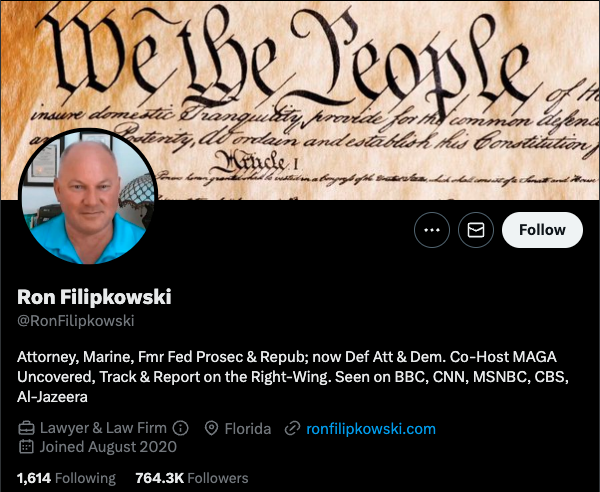
\includegraphics[width=1\columnwidth]{figures/ron.png}
\end{minipage}
\begin{minipage}[l]{0.45\textwidth}

\includegraphics[width=1\columnwidth]{figures/atrupar.png} 
\end{minipage}

\begin{minipage}[l]{1\textwidth}
\caption{Accounts like @ronfilipkowski and @atrupar had users of similar political orientations reply in a toxic manner to the news and opinions they tweeted.\label{fig:orientation-bio}}
\end{minipage}

\end{figure}



\begin{table}
\centering
\small
\begin{tabular}{l|rr}
%\toprule
\textbf{Account} &\textbf{\# Waves } & \textbf{Avg Partisanship of Wave } \\\midrule
@ronfilipkowski & 25  & -0.491\\
@youtube & 18 & 0.128\\
@elonmusk & 16 & 0.345 \\
@potus & 16 & 0.537\\
@repmtg & 14 & -0.366\\
@laurenboebert & 12 & 0.091\\
@acyn & 11& -0.766\\
@atrupar & 10 &-0.583\\
@donaldjtrumpjr & 10 & -0.131\\
@foxnews & 9 & -0.090\\
\bottomrule

\end{tabular}
\caption{\label{tab:campaigns} Number and average partisanship of toxic reply/mention waves encountered by various Twitter accounts.} 
\vspace{-15pt}
\end{table}
\vspace{2pt}
\noindent
\textbf{``Toxic Topics Waves.''} As was seen in our set of left-leaning topics, after examining the rest of our clusters, we observed several other separate instances when various users encountered ``toxic topics waves'' of toxic replies/mentions (\textit{i.e.}, where the majority of tweets were "@"s at a particular account).  For example, while we displayed one toxicity wave targeting Georgia Congresswoman Majorie Taylor Greene, we identified 13 other such toxicity waves in our dataset. For example, in one such wave, a user wrote:
\begin{displayquote}
\small
\textit{Oh wow RepMTG all the traitors together today!!!!  Could y'all imagine if the Obamas or Clinton's did this corrupt bullshit!!}
\end{displayquote}
while in another wave a different user wrote
\begin{displayquote}
\small
\textit{RepMTG Marge is a neanderthal idiot. No one is stupidly pushing drag queen shows or teaching gender lies - advocating "genital mutilation" ffs - what a bunch of ridiculous stupid! But hey, JAN 6 coup to sell the US to Russia, DANGER of losing our Democracy to extremists wacks!}
\end{displayquote}

Altogether we identified 4,506~toxicity waves against 3,822~users. 1,383 of these waves have a right-leaning orientation (\textit{i.e.}, average partisanship of toxicity wave participant > 0) while 3,123 have a liberal orientation. Calculating the political orientation of these ``attacked'' accounts, across these ``toxicity waves'', 14.5\% were in cases of right-leaning accounts campaigning against liberal accounts; 17.4\% were cases of liberal accounts campaigning against right-leaning accounts; 35.9\% were right-leaning against right-leaning; 33.5\% were left-leaning against left-leaning. Compared to all mentions where only 33.8\% are between users of different political orientations, we thus again observe evidence of affective polarization in these ``toxic topics waves.'' In Table~\ref{tab:campaigns}, we present the number of ``topics toxicity waves'' against particular users. 54.5\% (541 accounts) of the ``attacked'' accounts were verified (compared to only 10.7\% [4,610 accounts] of the accounts out dataset of 43,151 Twitter users),  suggesting that more public figures are more likely to incur these waves.

We note that, while in some cases these are targeted campaigns meant to attack particular users, in several cases these toxic waves are other Twitter accounts toxicly responding in agreement to the opinions or news put forward by the account. While the waves targeting @laurenboebert, a conservative congressperson from Colorado, are mostly by heavily left-leaning users for example, this occurs in reverse for two hyperpartisan liberal commentators user @atrupar and  @ronfilipkowski. For example in one such case, a user tweeted
\begin{displayquote}
\small
\textit{@RonFilipkowski Trump supporters are so dumb, they confuse antifa with nazis. There were nazis in Trump's White House.}
\end{displayquote}
Other waves, for instance, were aimed at @YouTube to protest particular videos being taken down.  

%We leave it to future work to fully explore and differentiate between these types of ``toxic topics waves.'' 



\clearpage
\newpage
\section{Most Toxic Topics \label{sec:most-toxic-by-percentage}}
\begin{table}[!h]
\centering
\scriptsize
\selectfont
\setlength{\tabcolsep}{4pt}
\begin{tabularx}{\textwidth}{l|XrXrXrrr}
\toprule
 &   &  &   \# Toxic & Avg.& Example & Avg.  & Avg. Partisan  & Partisan \\
 Topic& {Keywords}&\# Tweets &Tweets  & Toxicity &  Tweet  & Partisan. & of Toxic Users& Std. \\
\midrule

 1 & fuck, shit…, shit, shittttt, extremely &52 & 52 (100\%) &0.923 & That's all folks. Fuck this shit. &-0.169 &-0.167 & 0.737\\ 
2 & idiot, blitering, complete, total, he & 3121 & 3,123 (99.94\%) &0.915 & Not idiots. Deliberate enablers of fascism. &  0.152 & 0.128 & 0.970 \\
3& fuck, you, him, though, that's & 340 & 336 (98.82\%) &0.902& Fuck this and fuck him.& -0.027& -0.117 & 0.836 \\
4& piece, load, shit, hahahha, you &756 & 775 (97.55\%) &0.895 &   Tell me you are a piece of shit without telling me. & 0.011 &0.007& 0.957 \\
5&volume, youtube, chop, stupid, that & 435 & 438 (99.32\%) &0.880 & Nothing stupid about that!  & 0.119&0.104& 0.942 \\


\bottomrule
\end{tabularx}
\caption{\label{tab:narratives} Top toxic topics---by average toxic value---in our dataset.\label{table:toxic-topic-max}} 
\end{table}


\newpage
\section{Linear Fit of Topic-Level Features against Perspective Toxicity \label{sec:cluster-perspective-tox}}
\begin{figure}[!h]
\begin{minipage}[l]{1.0\textwidth}
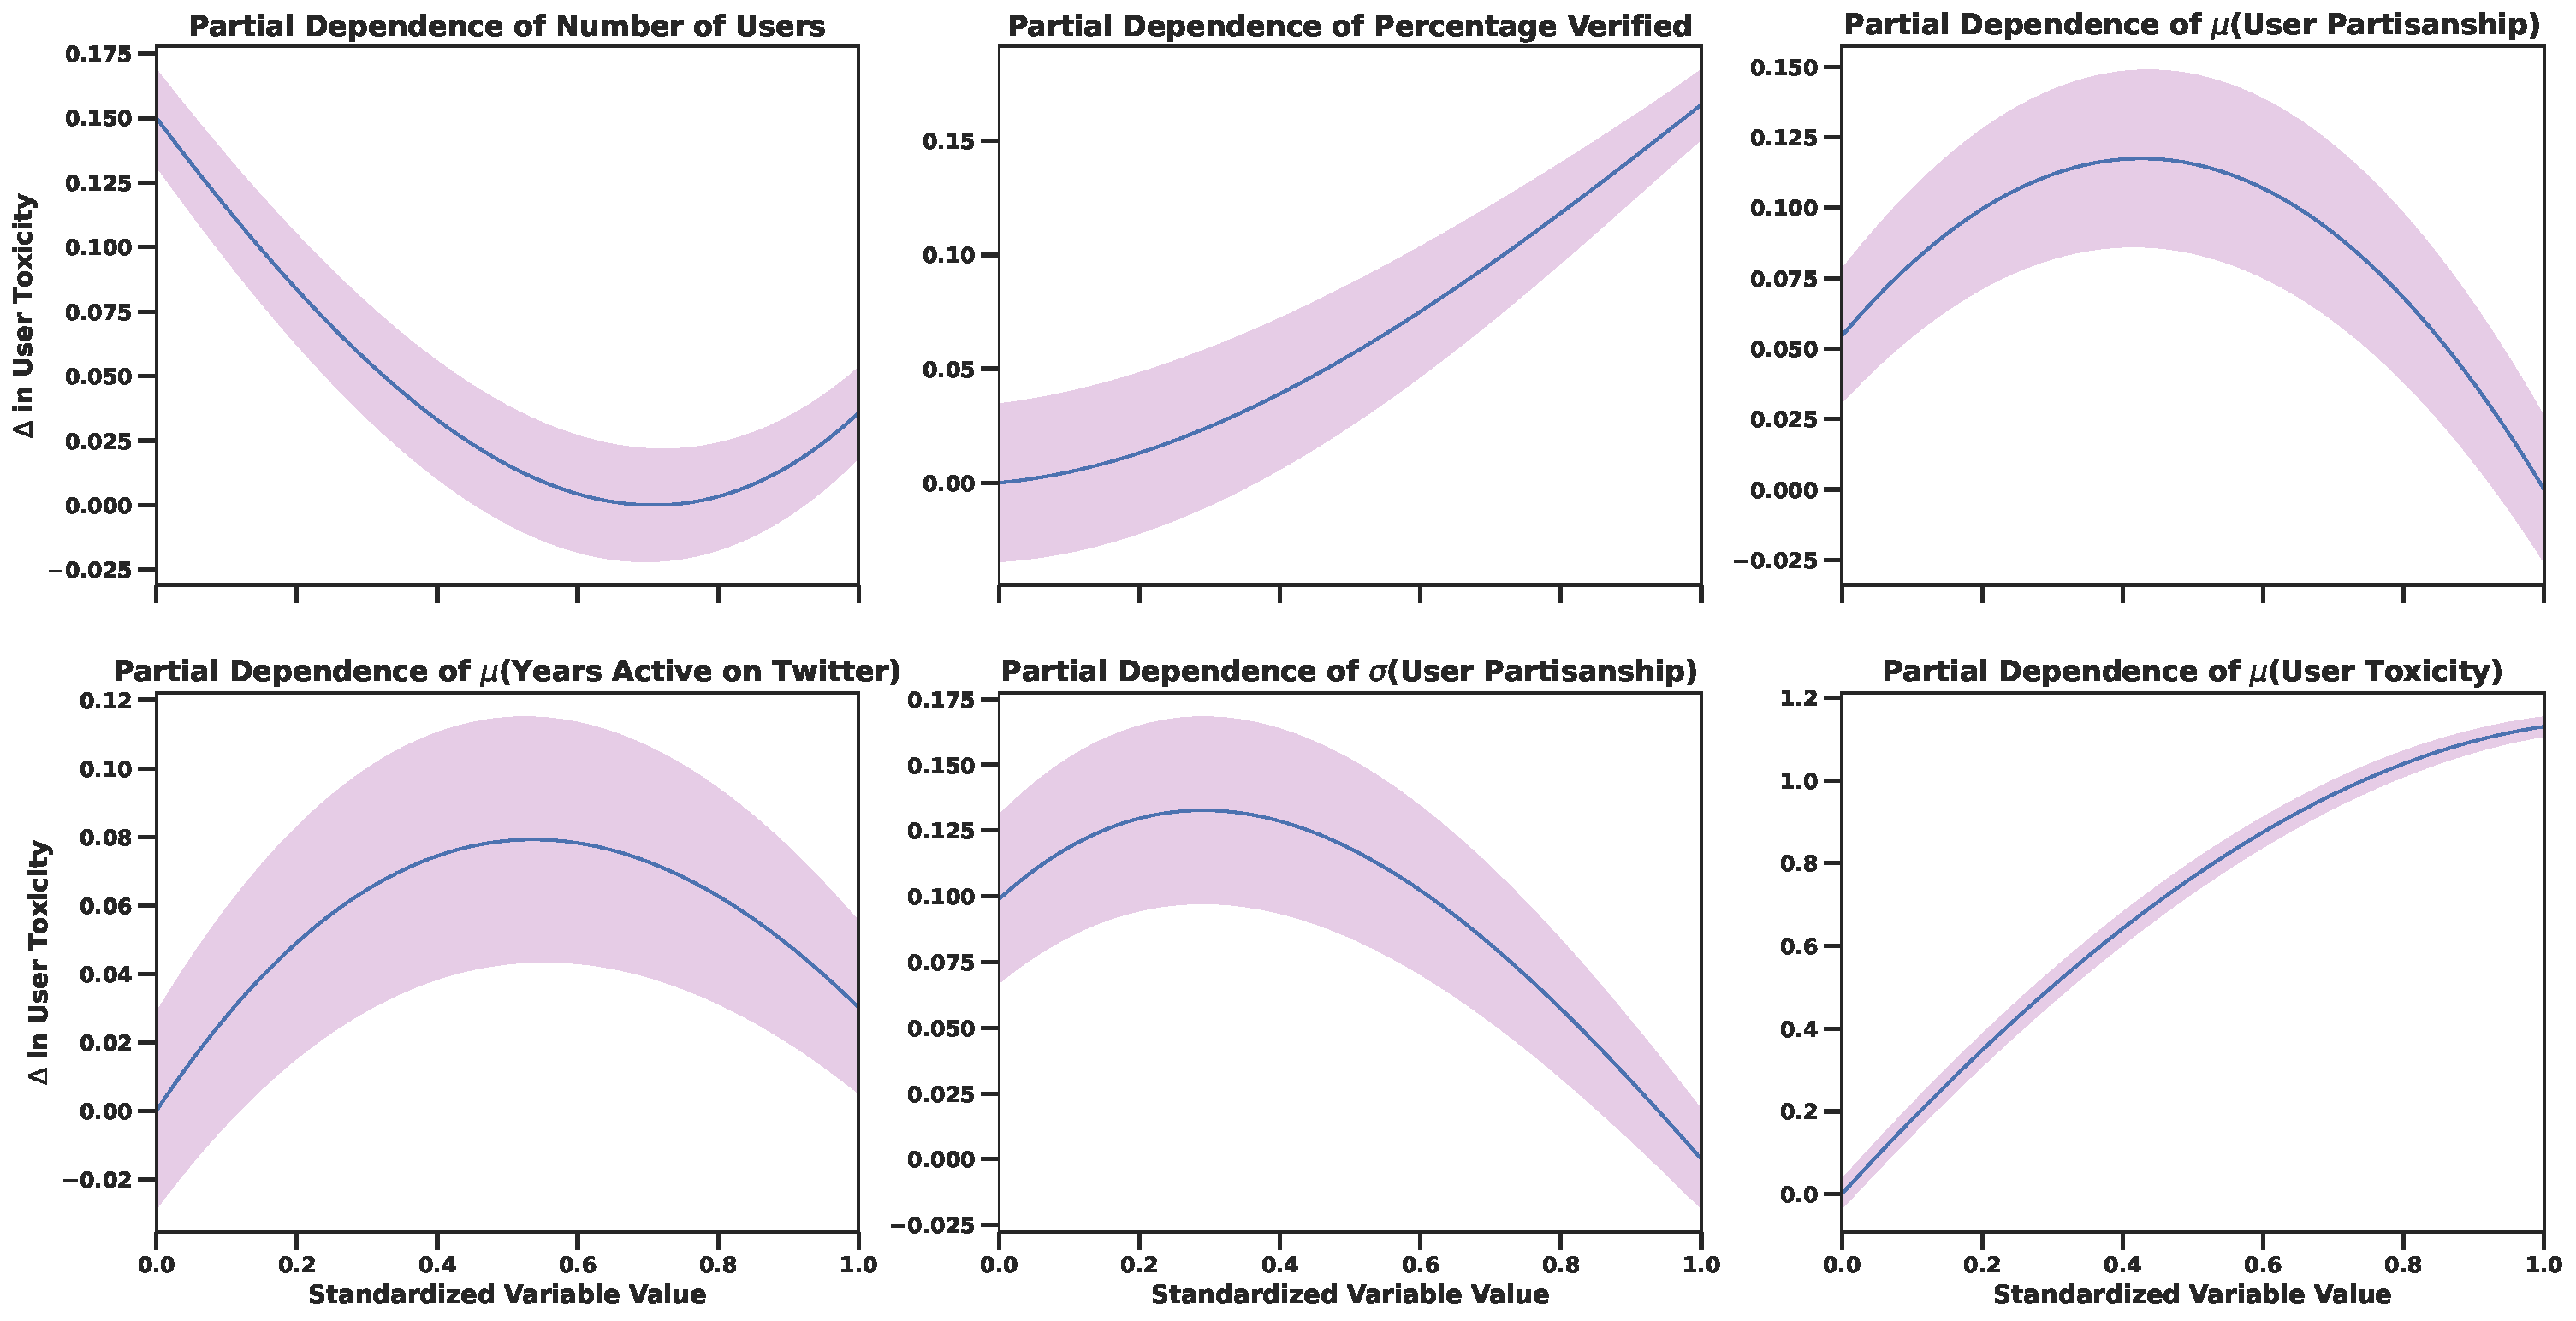
\includegraphics[width=1\columnwidth]{figures/partial_dependence_important_variables-clusterlevel-perspective.pdf} 
\end{minipage}
\begin{minipage}[l]{1\textwidth}
\caption{Partial dependencies with 95\% Normal Confidence intervals between fitted standardized dependent variables and cluster Perspective API toxicity.}
\end{minipage}
\end{figure}
\begin{table}[!h]
    \small
    \centering
    \begin{tabularx}{0.85\columnwidth}{l|rrr}
      Train $R^2$ 0.454, Validation $R^2$:  0.463  \\
    \toprule
      Dependent Variable  & Pearson Corr. $\rho$ & Kendall's $\tau$ & Permut Import. \\    \midrule
  Number of Users &-0.268 & -0.132  & 0.520  \\
 $\mu$(Years Active on Twitter) &-0.233 & -0.192 & 0.010\\
  Percentage Verified &0.273 & 0.247 & 0.014 \\
$\sigma$(User Partisanship) & -0.097 & -0.012 & 0.036 \\
  $\mu$|User Partisanship) & -0.014 &  0.011 & 0.013 \\
  $\mu$(User Toxicity) &  0.637 & 0.502 & 0.398 \\
    \bottomrule
    \end{tabularx}
  \caption{Pearson correlation $\rho$ and Kendall's $\tau$ of dependent variables and clusters' toxicities. } 
   \vspace{-15pt}
   \label{table:regression-20240402}
\end{table}
